\section{Measurement and Results}
As mentioned above, this experiment has 3 different sets of measurements: 
\begin{itemize}
    \item \textbf{Measurement of Correlation Functions}
    \item \textbf{Violation of Bell’s Inequality}
    \item \textbf{Quantum State Tomography}
\end{itemize}

Thus, this section is also divided into 3 different sections. Each subsection is dedicated to one of the following.

\subsection{Correlation Functions}
In the first part of the experiment, the aim is to measure correlation functions for 2 different cases. In both cases, there are 2 different half-wave plates. One half-wave plate ($HWP_{B}$) is located in the pathway of the photon that goes to Bob, and the other one ($HWP_{A}$) is located in the pathway of the photon that goes to Alice. The angles of the half-wave plates are as follows: 
\begin{itemize}
    \item {Case 1}:
        $\alpha_{HWP_{B}}$ = 0$^\circ$, $\alpha_{HWP_{A}}$ = $i^\circ$ ($i \in$ \{0, 10, 20, 30, 40, 50, 60, 70, 80, 90\})
    \item {Case 2}:
        $\alpha_{HWP_{B}}$ = 22.5$^\circ$, $\alpha_{HWP_{A}}$ = $i^\circ$ ($i \in$ \{0, 10, 20, 30, 40, 50, 60, 70, 80, 90\})
\end{itemize}
For both cases, the angles for the half-wave plates were changed by rotating the half-wave plate. After each configuration, coincidence counts were recorded by the help of a C++ script. Counts for each state and case can be seen below:

% Table for the coincidence counts for the first case
\begin{table}[h!]
    \centering
    \begin{tabular}{|c|c|c|c|c|c|c|c|c|c|c|}
        \hline
        $\alpha_{HWP_{A}}$ & 0$^\circ$ & 10$^\circ$ & 20$^\circ$ & 30$^\circ$ & 40$^\circ$ & 50$^\circ$ & 60$^\circ$ & 70$^\circ$ & 80$^\circ$ & 90$^\circ$ \\
        \hline
        $C_{HH}$ & 251 & 197 & 164 & 76 & 29 & 9 & 28 & 113 & 187 & 216 \\
        $C_{HV}$ & 6 & 18 & 67 & 133 & 196 & 195 & 173 & 111 & 45 & 8 \\
        $C_{VH}$ & 5 & 8 & 67 & 135 & 206 & 232 & 225 & 127 & 56 & 7 \\
        $C_{VV}$ & 205 & 199 & 165 & 73 & 22 & 10 & 36 & 88 & 162 & 234 \\
        \hline
    \end{tabular}
    \caption{Coincidence counts for the first case where $\alpha_{HWP_{B}}$ = 0$^\circ$.}
    \label{tab:coincidence_counts_case1}
\end{table}

\begin{table}[h!]
    \centering
    \begin{tabular}{|c|c|c|c|c|c|c|c|c|c|c|}
        \hline
        $\alpha_{HWP_{A}}$ & 0$^\circ$ & 10$^\circ$ & 20$^\circ$ & 30$^\circ$ & 40$^\circ$ & 50$^\circ$ & 60$^\circ$ & 70$^\circ$ & 80$^\circ$ & 90$^\circ$ \\
        \hline
        $C_{HH}$ & 101 & 161 & 167 & 139 & 108 & 42 & 14 & 25 & 48 & 111 \\
        $C_{HV}$ & 105 & 50 & 26 & 30 & 76 & 154 & 190 & 199 & 155 & 112 \\
        $C_{VH}$ & 86 & 45 & 18 & 42 & 91 & 167 & 186 & 180 & 126 & 82 \\
        $C_{VV}$ & 106 & 183 & 222 & 199 & 157 & 98 & 37 & 21 & 62 & 135 \\
        \hline
    \end{tabular}
    \caption{Coincidence counts for the second case where $\alpha_{HWP_{B}}$ = 22.5$^\circ$.}
    \label{tab:coincidence_counts_case2}
\end{table}

\subsubsection{Calculation of Correlation Functions}
\label{subsubsec:correlation_functions}
To calculate the correlation values, first we need to calculate relative frequencies for each state. Relative frequencies are calculated by dividing the coincidence counts by the total number of counts:
\begin{equation}
    f_{ij} = \frac{C_{ij}}{\sum_{i,j} C_{ij}} \quad (i,j \in \{H, V\})
\end{equation}

After calculating the relative frequencies, we can calculate the correlation values using the following formula with the relative frequencies from \hyperref[tab:coincidence_counts_case1]{Table \ref*{tab:coincidence_counts_case1}} and \hyperref[tab:coincidence_counts_case2]{Table \ref*{tab:coincidence_counts_case2}}:
\begin{equation}
    K_{ij}^{ex} = f_{HH} - f_{HV} - f_{VH} + f_{VV}
\end{equation}
with $i, j \in \{H, V\}$. Correlation values for both cases can be seen below:
\begin{table}[h!]
    \centering
    \begin{tabular}{|c|c|c|c|c|c|c|c|c|c|c|}
        \hline
        $\alpha_{HWP_{A}}$ & 0$^\circ$ & 10$^\circ$ & 20$^\circ$ & 30$^\circ$ & 40$^\circ$ & 50$^\circ$ & 60$^\circ$ & 70$^\circ$ & 80$^\circ$ & 90$^\circ$ \\
        \hline
        $Case~1$ & 0.953 & 0.877 & 0.421 & -0.279 & -0.775 & -0.915 & -0.723 & -0.084 & 0.551 & 0.936 \\ 
        $Case~2$ & 0.040 & 0.567 & 0.797 & 0.648  & 0.227  & -0.393 & -0.761 & -0.784 & -0.437 & 0.118 \\
        \hline
    \end{tabular}
    \caption{Calculated correlation values.}
    \label{tab:correlation_values}
\end{table}

The relation between the correlation values and the angles can be visualized by plotting the correlation values against the angles. Since the correlation values are sinusoidal functions, we can fit the correlation values to a sinusoidal function. The fits for both cases can be seen below:
\begin{figure}[h!]
    \centering
    \begin{subfigure}[t]{0.45\textwidth}
        \centering
        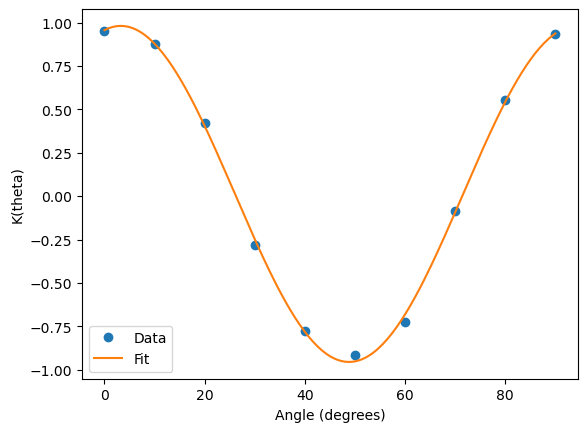
\includegraphics[width=\textwidth]{figures/fit_1.png}
        \caption{Case 1.}
        \label{fig:fit_1}
    \end{subfigure}
    \hfill
    \begin{subfigure}[t]{0.45\textwidth}
        \centering
        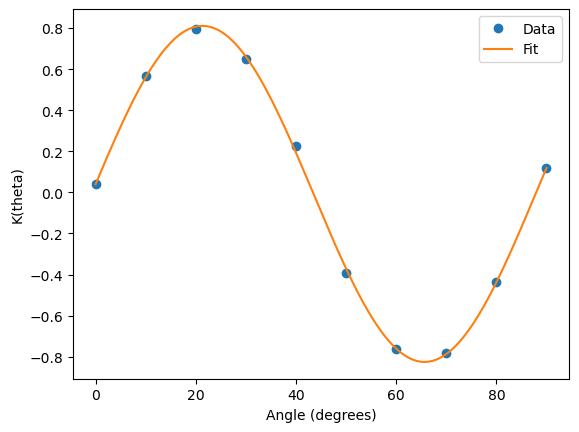
\includegraphics[width=\textwidth]{figures/fit_2.png}
        \caption{Case 2.}
        \label{fig:fit_2}
    \end{subfigure}
    \caption{Correlation values for both cases. 
        $f(\theta) = A \cdot \sin(B \cdot \theta + C) + D$ is used as the fit function.
    }
    \label{fig:fit_comparison}
\end{figure}

\subsubsection{Visibility}
The visibility can be used to parameterize the contrast of measured graphs \cite{manual}. It is defined as the ratio of the difference between the maximum and minimum value of the correlation function to the sum of the maximum and minimum values.
Since a correlation function can be bounded by -1 and 1, the visibility of this function would lead to $\frac{2}{0}$ in a perfect experimental setup. 
To deduce the visibility of the correlation function, we can use a fit function that maps a flat correlation function to 0 and a sinusoidal correlation function to 1.
This can be easily achieved by using the following formula:
\[\mathcal{V} = \frac{\max_{\theta} \tilde{f}(\theta) - \min_{\theta} \tilde{f}(\theta)}{2}\]

This formula will result in a value between 0 and 1, where 0 indicates a flat correlation function and 1 indicates a correlation function varrying between -1 and 1. By using this formula, we can calculate the visibility of the correlation functions for both cases.
{\itshape Case 1} has a visibility of 0.934, while {\itshape Case 2} has a visibility of 0.791.

\subsubsection{Necessity of Two Correlation Functions}
In this experiment, (as any other Bell test experiment) two correlation functions are needed to detect entanglement. Entanglement is a quantum correlation and to be able to detect it, 
we need to detect correlations (measuring correlation functions) in at least two different bases. Just measuring the correlation in one basis is not enough to detect entanglement, since 
correlations in one basis can be explained by classical correlations and local hidden variables\cite{bell,chsh}.  


\subsection{Violation of Bell’s Inequality}
In the second part of the experiment, the aim is to demonstrate the violation of CHSH inequality which is a generalization of Bell's theorem\cite{chsh}. As in the first part of the experiment
here we also have one half-wave plate for each party. Unlike the first part, we only have 4 sets of angles for the half-wave plates. The angles are as follows:

\begin{table}[h!]
    \centering
    \begin{tabular}{|c|c|c|c|}
        \hline
        \multicolumn{2}{|c|}{Alice} & \multicolumn{2}{c|}{Bob} \\ \hline
        $\alpha$ & $\alpha'$ & $\beta$ & $\beta'$ \\ \hline
        $22.5^\circ$ & $0^\circ$ & $11.25^\circ$ & $-11.25^\circ$ \\ \hline
    \end{tabular}
    \caption{Measurement settings for Alice and Bob.}
    \label{tab:measurement_settings}
\end{table}



Experimental settings for Alice and Bob’s angles.

Calculation of correlation functions and error propagation.

Interpretation of results demonstrating Bell inequality violation.

\subsection{Quantum State Tomography}
Measurement procedure for the four Bell states (\(|\phi^+\rangle\), \(|\phi^-\rangle\), \(|\psi^+\rangle\), \(|\psi^-\rangle\)).

Reconstruction of density matrices from experimental data.

Calculation of fidelity, purity, and eigenvalues.

Proof of entanglement using PPT criterion and entanglement witnesses.